% !TeX program = xelatex
\documentclass[runningheads]{llncs}
\usepackage[paperheight=295mm,paperwidth=210mm]{geometry}
\usepackage{graphicx}
\usepackage{wrapfig}
\usepackage{import}
\usepackage{kotex}
\usepackage[dvipsnames]{xcolor}
\usepackage{fancyvrb} %
\usepackage{listings}
\usepackage{tabularx}
\usepackage{underscore}
\usepackage{multicol}
\usepackage{enumitem}
\usepackage{subcaption}
\usepackage[numbers,square,super]{natbib}
\usepackage{mathptmx} % Times New Roman
\usepackage{amsmath}
\usepackage{amssymb}
\usepackage{framed}
\usepackage{etoolbox}
\usepackage{cancel}
\usepackage{physics}
\usepackage{tikz}
\usepackage{parskip}
\usepackage{enumerate}
\usepackage{minted}
\usepackage{inconsolata}
\usepackage{makecell}
\usepackage{slashed}
\usepackage{nicematrix}
\usetikzlibrary{calc, angles, quotes, graphs, positioning, arrows}

\setcounter{tocdepth}{2}

\colorlet{shadecolor}{gray!30}

\newcommand\enclosebox[2]{%
  \BeforeBeginEnvironment{#1}{\begin{#2}}%
  \AfterEndEnvironment{#1}{\end{#2}}%
}

\enclosebox{theorem}{oframed}
\enclosebox{definition}{leftbar}

\newcommand{\divides}{\bigm|}
\newcommand{\ndivides}{%
  \mathrel{\mkern.5mu % small adjustment
    % superimpose \nmid to \big|
    \ooalign{\hidewidth$\big|$\hidewidth\cr$\nmid$\cr}%
  }%
}
\newcommand{\ord}{\operatorname{\mathrm{ord}}}
\newcommand{\ind}{\operatorname{\mathrm{ind}}}
\newcommand{\legendre}[2]{\left(\frac{#1}{#2}\right)}
\setmainfont{Times New Roman}
\setmainhangulfont{Nanum Myeongjo}
\setmonofont{SF Mono}
\setlength{\parindent}{1em}
\setlength{\parskip}{0pt}
\linespread{1.2}
%\renewcommand{\arraystretch}{1.5}
\setlength{\tabcolsep}{0.5em}%
\newenvironment{Figure}
  {\par\medskip\noindent\minipage{\linewidth}}
  {\endminipage\par\medskip}
\newcommand{\translation}[1]{\textsuperscript{#1}}

\makeatletter
\renewcommand\NAT@citesuper[3]{\ifNAT@swa
\if*#2*\else#2\NAT@spacechar\fi
\unskip\kern\p@\textsuperscript{\NAT@@open#1\if*#3*\else,\NAT@spacechar#3\fi\NAT@@close}%
   \else #1\fi\endgroup}
\makeatother

\let\oldtabular\tabular% Store a copy of \tabular
\let\endoldtabular\endtabular% Store a copy of \endtabular
\renewenvironment{tabular}[2][\arraystretch]
  {\edef\arraystretch{#1}% Update \arraystretch
   \oldtabular{#2}}% \begin{tabular}[<stretch>]{<col spec>}
  {\endoldtabular}% \end{tabular}

\begin{document}

\title{Linear Algebra (0031)\newline\space Problem Set 1 Solutions}
\author{Yulwon Rhee (202211342)}
\institute{Department of Computer Science and Engineering, Konkuk University}

\maketitle
\subsubsection{1.}
(a) Calculate $b_{11}\mathbf{a}_1+b_{21}\mathbf{a}_2$.
\paragraph{Solution.}
\begin{align*}
    b_{11}\mathbf{a}_1+b_{21}\mathbf{a}_2 &= \begin{bmatrix}
        2\\1\\3
    \end{bmatrix} + 2\begin{bmatrix}
        3\\-1\\1
    \end{bmatrix}\\
    &= \begin{bmatrix}
        8\\-1\\5
    \end{bmatrix}
\end{align*}\\

(b) Calculate $A\mathbf{b}_1$. Compare and discuss the results in parts (a) and (b).
\paragraph{Solution.}
\begin{align*}
    A\mathbf{b}_1 &= \begin{bmatrix}
        2&3\\1&-1\\3&1
    \end{bmatrix} \begin{bmatrix}
        1\\2
    \end{bmatrix}\\ &= \begin{bmatrix}
        8\\-1\\5
    \end{bmatrix}
\end{align*}
$$\therefore b_{11}\mathbf{a}_1+b_{21}\mathbf{a}_2=A\mathbf{b}_1$$\\
Multiplication between matrix and column vector is defined so that the entry $(i, j)$ of the product is the dot product of the
left matrix's row $i$ and the right column vector's column $j$. So, $A\mathbf{b}_1$ is calculated as same as $b_{11}\mathbf{a}_1+b_{21}\mathbf{a}_2$\\

(c) Calculate $a_{11}\mathbf{b}_1+a_{12}\mathbf{b}_2$.
\paragraph{Solution.}
\begin{align*}
    a_{11}\mathbf{b}_1+a_{12}\mathbf{b}_2 &= 2\begin{bmatrix}
        1&3
    \end{bmatrix} + 3\begin{bmatrix}
        2&3
    \end{bmatrix}\\&=\begin{bmatrix}
        8&15
    \end{bmatrix}
\end{align*}
\newpage
(d) Calculate $\underline{\mathbf{a}}_1B$. Compare and discuss the results in parts (c) and (d).
\paragraph{Solution.}
\begin{align*}
    \underline{\mathbf{a}}_1B &= \begin{bmatrix}
        2&3
    \end{bmatrix}\begin{bmatrix}
        1&3\\2&3
    \end{bmatrix}\\&=\begin{bmatrix}
        8&15
    \end{bmatrix}
\end{align*}
$$\therefore a_{11}\mathbf{b}_1+a_{12}\mathbf{b}_2 = \underline{\mathbf{a}}_1B$$\\
Multiplication between row vector and matrix is defined so that the entry $(i, j)$ of the product is the dot product of the
left row vector's row $i$ and the right matrix's column $j$. So, $\underline{\mathbf{a}}_1B$ is calculated as same as $a_{11}\mathbf{b}_1+a_{12}\mathbf{b}_2$\\

(e) Calculate $\begin{bmatrix}
    \underline{\mathbf{a}}_1B\\
    \underline{\mathbf{a}}_2B\\
    \underline{\mathbf{a}}_3B
\end{bmatrix}$.
\paragraph{Solution.}
\begin{align*}
    \underline{\mathbf{a}}_2B &= \begin{bmatrix}
        1&-1
    \end{bmatrix}\begin{bmatrix}
        1&3\\2&3
    \end{bmatrix}\\&=\begin{bmatrix}
        -1&0
    \end{bmatrix}\\
    \underline{\mathbf{a}}_3B &= \begin{bmatrix}
        3&1
    \end{bmatrix}\begin{bmatrix}
        1&3\\2&3
    \end{bmatrix}\\&=\begin{bmatrix}
        5&12
    \end{bmatrix}
\end{align*}\\
$$\therefore \begin{bmatrix}
    \underline{\mathbf{a}}_1B\\
    \underline{\mathbf{a}}_2B\\
    \underline{\mathbf{a}}_3B
\end{bmatrix} = \begin{bmatrix}
    8&15\\-1&0\\5&12
\end{bmatrix}(\because \text{(d)})$$\\
\newpage
(f) Calculate $\begin{bmatrix}
    A\mathbf{b}_1&A\mathbf{b}_2
\end{bmatrix}$.
\paragraph{Solution.}
\begin{align*}
    A\mathbf{b}_2 &= \begin{bmatrix}
        2&3\\1&-2\\3&1
    \end{bmatrix}\begin{bmatrix}
        3\\3
    \end{bmatrix}\\&=\begin{bmatrix}
        15\\0\\12
    \end{bmatrix}
\end{align*}\\
$$\begin{bmatrix}
    A\mathbf{b}_1&A\mathbf{b}_2
\end{bmatrix} = \begin{bmatrix}
    8&15\\-1&0\\5&12
\end{bmatrix} (\because \text{(b)})$$\\

(g) Calculate $AB$.
\paragraph{Solution.}
\begin{align*}
    AB &= \begin{bmatrix}
        2&3\\1&-1\\3&1
    \end{bmatrix}\begin{bmatrix}
        1&3\\2&3
    \end{bmatrix}\\
    &=\begin{bmatrix}
        8&15\\-1&0\\5&12
    \end{bmatrix}
\end{align*}\\

(h) Using all the results in parts (e), (f) and (g), discuss how matrix multiplication can be interpreted.
\paragraph{Solution.}
By the results in parts (e), (f) and (g), Multiplication between two vectors can be factored into the multiplication between row vectors of matrix and another matrix, or the multiplication between the matrix and column vectors of another matrix.
\newpage
\subsubsection{2.} Find a $4\times4$ permutation matrix $P\neq I$ satisfying $P^3 = I$.
\paragraph{Solution.}
By the python code below, you can find all possible cases of $P$ using Brute Force Algorithm.\\
\begin{minted}[linenos, fontsize=\small]{python}
import itertools
import numpy as np
I = np.identity(4)
cases = list(itertools.permutations(I))

for case in cases:
    P = np.array(case)
    # @ means matrix multiplication in numpy
    if np.array_equal(P @ P @ P, I) and not np.array_equal(P, I):
        print(P)
\end{minted}

So, $P$ can be $\begin{bmatrix}
    1&0&0&0\\0&0&1&0\\0&0&0&1\\0&1&0&0
\end{bmatrix}, \begin{bmatrix}
    1&0&0&0\\0&0&0&1\\0&1&0&0\\0&0&1&0
\end{bmatrix}, \begin{bmatrix}
    0&1&0&0\\0&0&1&0\\1&0&0&0\\0&0&0&1
\end{bmatrix}, \begin{bmatrix}
    0&1&0&0\\0&0&0&1\\0&0&1&0\\1&0&0&0
\end{bmatrix}, \begin{bmatrix}
    0&0&1&0\\1&0&0&0\\0&1&0&0\\0&0&0&1
\end{bmatrix}, \begin{bmatrix}
    0&0&1&0\\0&1&0&0\\0&0&0&1\\1&0&0&0
\end{bmatrix}, \begin{bmatrix}
    0&0&0&1\\1&0&0&0\\0&0&1&0\\0&1&0&0
\end{bmatrix}, \begin{bmatrix}
    0&0&0&1\\0&1&0&0\\1&0&0&0\\0&0&1&0
\end{bmatrix}$.
\newpage
\subsubsection{3.}
(a) Consider an $m\times n$ matrix $A$ and a column vector $\mathbf{x} \in \mathbb{R}^n$.
We know that $A\mathbf{x}$ is a combination of columns of $A$. Give an interpretation of the multiplication $\mathbf{x}^T A^T$.
\paragraph{Solution.}
Let $A = \begin{bmatrix}
    a_{11} & a_{12} & \cdots & a_{1n}\\
    a_{21} & a_{22} & \cdots & a_{2n}\\
    \vdots & \vdots & \ddots & \vdots\\
    a_{m1} & a_{m2} & \cdots & a_{mn}
\end{bmatrix}$ and $\mathbf{x} = \begin{bmatrix}
    x_1\\x_2\\\vdots\\x_n
\end{bmatrix}$.
\begin{align*}
    \mathbf{x}^TA^T &= \begin{bmatrix}
        x_1&x_2&\cdots&x_n
    \end{bmatrix}\begin{bmatrix}
        a_{11} & a_{21} & \cdots & a_{m1}\\
        a_{12} & a_{22} & \cdots & a_{m2}\\
        \vdots & \vdots & \ddots & \vdots\\
        a_{1n} & a_{2n} & \cdots & a_{mn}
    \end{bmatrix}\\
    &= \begin{bmatrix}
        a_{11}x_1 + a_{12}x_2 + \cdots + a_{1n}x_n\quad\quad
        a_{21}x_1 + a_{22}x_2 + \cdots + a_{2n}x_n\quad
        \cdots\quad
        a_{m1}x_1 + a_{m2}x_2 + \cdots + a_{mn}x_n
    \end{bmatrix}
\end{align*}\\

(b) Argue that $(A\mathbf{x})^T = \mathbf{x}^T A^T$.
\paragraph{Solution.}
We know that $A\mathbf{x}$ is a combination of columns of $A$.\\

i.e., $A\mathbf{x} = \begin{bmatrix}
    a_{11}x_1 + a_{12}x_2 + \cdots + a_{1n}x_n\\
    a_{21}x_1 + a_{22}x_2 + \cdots + a_{2n}x_n\\
    \vdots\\
    a_{m1}x_1 + a_{m2}x_2 + \cdots + a_{mn}x_n
\end{bmatrix}$.\\
$\therefore(A\mathbf{x})^T = \begin{bmatrix}
    a_{11}x_1 + a_{12}x_2 + \cdots + a_{1n}x_n\quad\quad
    a_{21}x_1 + a_{22}x_2 + \cdots + a_{2n}x_n\quad
    \cdots\quad
    a_{m1}x_1 + a_{m2}x_2 + \cdots + a_{mn}x_n
\end{bmatrix}$.\\

$$\therefore (A\mathbf{x})^T = \mathbf{x}^T A^T$$\\

(c) Consider an $n\times p$ matrix $B$.
Let $B=\begin{bmatrix}
    \mathbf{b}_1 & \mathbf{b}_2 & \cdots & \mathbf{b}_p
\end{bmatrix}$.
We know $AB=􏰀\begin{bmatrix}
    A\mathbf{b}_1 & A\mathbf{b}_2 & \cdots & A\mathbf{b}_p
\end{bmatrix}$.
Take the transpose of $AB$ and show that $(AB)^T = B^T A^T$.
\paragraph{Solution.}
% \begin{align*}
%     (AB)^T &= \begin{bmatrix}
%         (A\mathbf{b}_1)^T\\
%         (A\mathbf{b}_2)^T\\
%         \vdots\\
%         (A\mathbf{b}_p)^T\\
%     \end{bmatrix}\\
%     &= \begin{bmatrix}
%         \mathbf{b}_1^TA^T\\
%         \mathbf{b}_2^TA^T\\
%         \vdots\\
%         \mathbf{b}_p^TA^T\\
%     \end{bmatrix} (\because (A\mathbf{x})^T = \mathbf{x}^T A^T)\\
% \end{align*}
% $$B^T = \begin{bmatrix}
%     \mathbf{b}_1^T\\
%     \mathbf{b}_2^T\\
%     \vdots\\
%     \mathbf{b}_p^T\\
% \end{bmatrix}$$
% $$B^TA^T = \begin{bmatrix}
%     \mathbf{b}_1^TA^T\\
%     \mathbf{b}_2^TA^T\\
%     \vdots\\
%     \mathbf{b}_p^TA^T\\
% \end{bmatrix}$$
% $$\therefore (AB)^T = B^TA^T$$
$$(AB)^T_{ij}=(AB)_{ji}=\sum^n_{k=1}A_{jk}B_{ki}$$
$$(B^TA^T)_{ij} = \sum^n_{k=1}B^T_{ik}A^T_{kj}=\sum^n_{k=1}B_{ki}A_{jk}=\sum^n_{k=1}A_{jk}B_{ki}$$\\
So, since $(AB)^T_{ij}=(B^TA^T)_{ij}$ for all $i = 1, 2, \cdots, p$ and $j = 1, 2, \cdots, m$ we have
$(AB)^T=B^TA^T$.
\newpage
\subsubsection{4.}
(a) Express the vector $\mathbf{x}$ as a function of $r$ and $\alpha$.
\paragraph{Solution.}
$$\mathbf{x} = \begin{bmatrix}
    r\cos\alpha\\r\sin\alpha
\end{bmatrix}$$\\

(b) Express the vector $\mathbf{y}$ as a function of $r,\theta,\alpha$.
\paragraph{Solution.}
$$\mathbf{y} = \begin{bmatrix}
    r\cos(\alpha+\theta)\\r\sin(\alpha+\theta)
\end{bmatrix}$$\\

(c) Based on the expressions in parts (a) and (b), what is the matrix $R_o(\theta)$ such that $\mathbf{y}=R_o(\theta)\mathbf{x}$
\paragraph{Solution.}
Let $R_o(\theta) = \begin{bmatrix}
    \cos\theta & -\sin\theta\\
    \sin\theta & \cos\theta
\end{bmatrix}$.
\begin{align*}
    R_o(\theta)\mathbf{x} &= \begin{bmatrix}
        \cos\theta & -\sin\theta\\
        \sin\theta & \cos\theta
    \end{bmatrix} \begin{bmatrix}
        r\cos\alpha\\r\sin\alpha
    \end{bmatrix}\\
    &= \begin{bmatrix}
        r\cos\theta\cos\alpha - r\sin\theta\sin\alpha\\
        r\sin\theta\cos\alpha + r\cos\theta\sin\alpha
    \end{bmatrix}\\
    &= \begin{bmatrix}
        r\cos(\alpha+\theta)\\r\sin(\alpha+\theta)
    \end{bmatrix} (\because \text{Angle Addition and Subtraction Formulas})\\
    &= \mathbf{y}
\end{align*}
$$\therefore R_o(\theta) = \begin{bmatrix}
    \cos\theta & -\sin\theta\\
    \sin\theta & \cos\theta
\end{bmatrix}$$
\newpage
(d) Show that $R_o(\theta)\mathbf{x}$ and $\mathbf{x}$ have the same length.
\paragraph{Solution.}
$$\mathbf{y}=R_o(\theta)\mathbf{x}$$
\begin{align*}
    ||\mathbf{y}|| &= \sqrt{\mathbf{y}\cdot\mathbf{y}}\\
    &= \sqrt{\mathbf{y}^T\mathbf{y}}\\
    &= \sqrt{\{R_o(\theta)\mathbf{x}\}^TR_o(\theta)\mathbf{x}}\\
    &= \sqrt{\mathbf{x}^T\{R_o(\theta)\}^TR_o(\theta)\mathbf{x}}\\
    &= \sqrt{\mathbf{x}^TI\mathbf{x}}\\
    &= \sqrt{\mathbf{x}^T\mathbf{x}}\\
    &= ||\mathbf{x}||\\\tag*{$\qed$}
\end{align*}

(e) Describe what $R_o(\frac{\pi}{2})$ does when $R_o(\frac{\pi}{2})$ is multiplied on the vector $\mathbf{x}$.
\paragraph{Solution.}
\begin{align*}
    R_o\left( \frac{\pi}{2} \right)\mathbf{x} &= \begin{bmatrix}
        \cos\frac{\pi}{2} & -\sin\frac{\pi}{2}\\
        \sin\frac{\pi}{2} & \cos\frac{\pi}{2}\\
    \end{bmatrix}\begin{bmatrix}
        r\cos\alpha\\r\sin\alpha
    \end{bmatrix}\\
    &=\begin{bmatrix}
        0 & -1\\1&0
    \end{bmatrix} \begin{bmatrix}
        r\cos\alpha\\r\sin\alpha
    \end{bmatrix}\\
    &= \begin{bmatrix}
        -r\sin\alpha\\r\cos\alpha
    \end{bmatrix}
\end{align*}
\begin{gather*}
    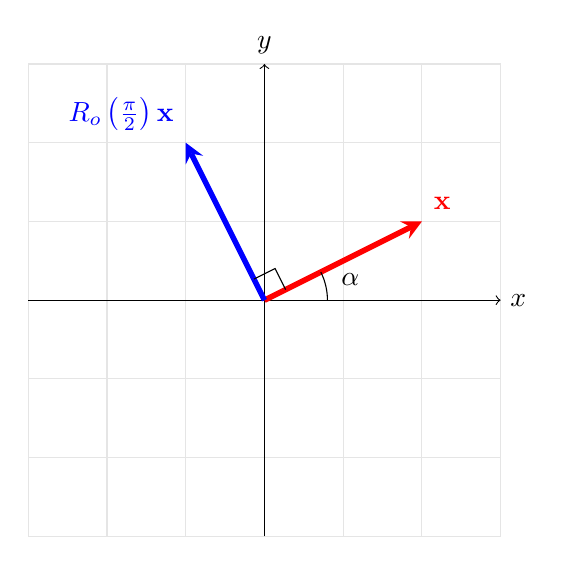
\begin{tikzpicture}
        \coordinate (O) at (0,0);
        \coordinate (x) at (2,1);
        \coordinate (rox) at (-1,2);
        \coordinate (xaxis) at (3, 0);
        \draw[thin,gray!20] (-3,-3) grid (3,3);
        \draw[->] (-3,0)--(3,0) node[right]{$x$};
        \draw[->] (0,-3)--(0,3) node[above]{$y$};
        \draw[line width=2pt,red,-stealth](0,0)--(2,1) node[anchor=south west]{$\mathbf{x}$};
        \draw[line width=2pt,blue,-stealth](0,0)--(-1,2) node[anchor=south east]{$R_o\left( \frac{\pi}{2} \right)\mathbf{x}$};
        \pic [draw, angle radius = .3cm] {right angle = x--O--rox};
        \pic [draw, "$\alpha$", angle eccentricity=1.4, angle radius = .8cm] {angle = xaxis--O--x};
    \end{tikzpicture}
\end{gather*}
As you can see, $R_o\left( \frac{\pi}{2} \right)$ rotates vector $\mathbf{x}$ by $\frac{\pi}{2}$ when it is multiplied on the vector $\mathbf{x}$.

\subsubsection{5.}
(a) Express the vector $\mathbf{x}$ as a function of $r$ and $\alpha$.
\paragraph{Solution.}
$$\mathbf{x} = \begin{bmatrix}
    r\cos\alpha\\r\sin\alpha
\end{bmatrix}$$

(b) Express the vector $\mathbf{y}$ as a function of $r,\theta,\alpha$.
\paragraph{Solution.}
$$\mathbf{y} = \begin{bmatrix}
    r\cos(2\theta-\alpha)\\r\sin(2\theta-\alpha)
\end{bmatrix}$$

(c) Based on the expressions in parts (a) and (b), what is the matrix $R_e(\theta)$ such that $\mathbf{y}=R_e(\theta)\mathbf{x}$
\paragraph{Solution.}
Let $R_e(\theta) = \begin{bmatrix}
    \cos(2\theta) & \sin(2\theta)\\
    \sin(2\theta) & -\cos(2\theta)
\end{bmatrix}$.
\begin{align*}
    R_e(\theta)\mathbf{x} &= \begin{bmatrix}
        \cos(2\theta) & \sin(2\theta)\\
        \sin(2\theta) & -\cos(2\theta)
    \end{bmatrix} \begin{bmatrix}
        r\cos\alpha\\r\sin\alpha
    \end{bmatrix}\\
    &= \begin{bmatrix}
        r\cos(2\theta)\cos\alpha + r\sin(2\theta)\sin\alpha\\
        r\sin(2\theta)\cos\alpha - r\cos(2\theta)\sin\alpha
    \end{bmatrix}\\
    &= \begin{bmatrix}
        r\cos(2\theta-\alpha)\\r\sin(2\theta-\alpha)
    \end{bmatrix} (\because \text{Angle Addition and Subtraction Formulas})\\
    &= \mathbf{y}
\end{align*}
$$\therefore R_e(\theta) = \begin{bmatrix}
    \cos(2\theta) & \sin(2\theta)\\
    \sin(2\theta) & -\cos(2\theta)
\end{bmatrix}$$

(d) Draw the triangle formed by the columns of the matrix $A = \begin{bmatrix}
    1 & 2 & 1\\4 & 4 & 7
\end{bmatrix}$.
\begin{gather*}
    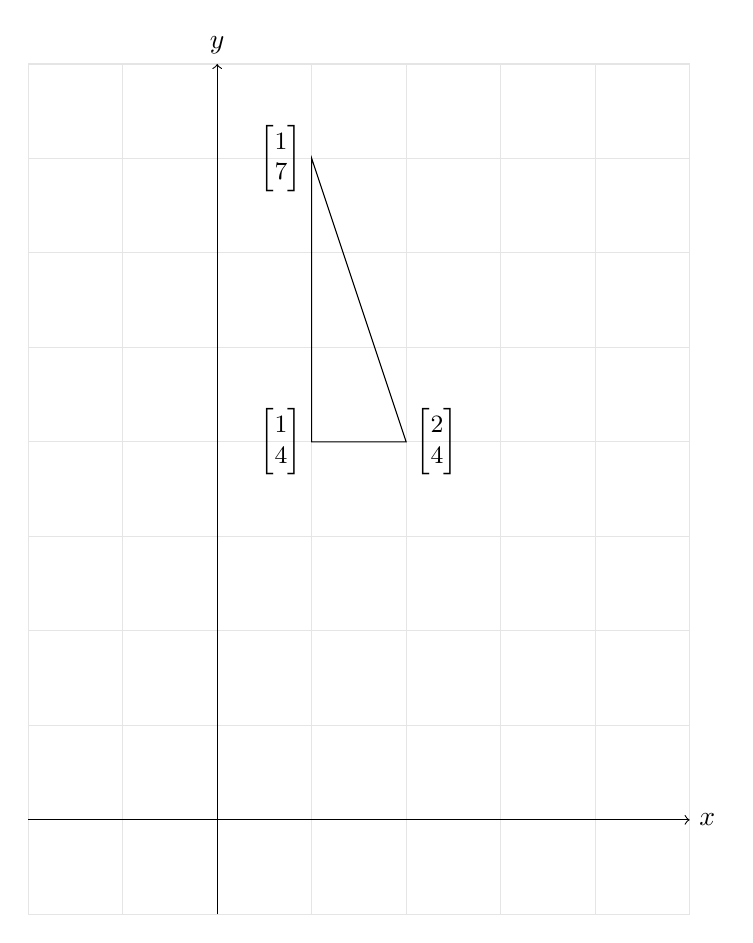
\begin{tikzpicture} [scale = 1.2]
        \coordinate (O) at (0,0);
        \draw[thin,gray!20] (-2, -1) grid (5,8);
        \draw[->] (-2,0)--(5,0) node[right]{$x$};
        \draw[->] (0,-1)--(0,8) node[above]{$y$};
        \draw (1,4) node[anchor=east]{$\small\begin{bmatrix}1\\4\end{bmatrix}$}
        -- (2,4) node[anchor=west]{$\small\begin{bmatrix}2\\4\end{bmatrix}$}
        -- (1,7) node[anchor=east]{$\small\begin{bmatrix}1\\7\end{bmatrix}$}
            -- cycle;
    \end{tikzpicture}
\end{gather*}

\pagebreak
(e) Draw the triangle formed by the columns of $R_e(0)A$.
\begin{align*}
    R_e(0)A &= \begin{bmatrix}
        1&0\\0&-1
    \end{bmatrix} \begin{bmatrix}
        1 & 2 & 1\\4 & 4 & 7
    \end{bmatrix}\\&= \begin{bmatrix}
        1 & 2 & 1\\-4 & -4 & -7
    \end{bmatrix}
\end{align*}
\begin{gather*}
    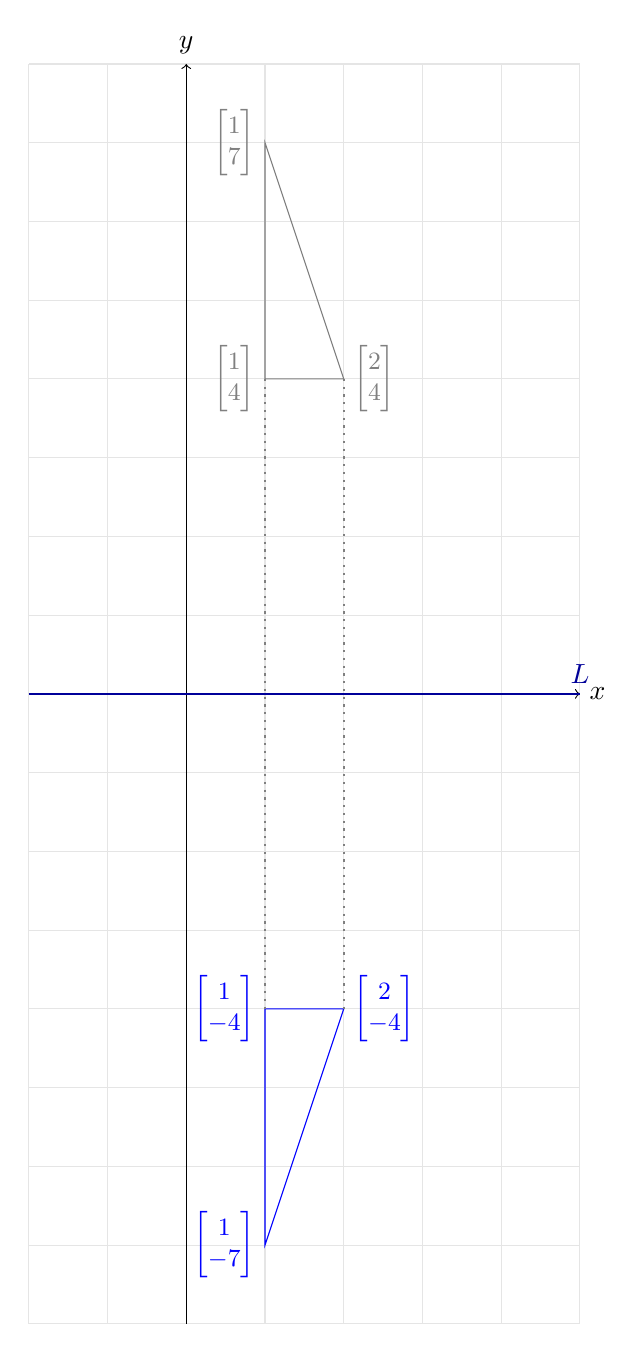
\begin{tikzpicture}
        \coordinate (O) at (0,0);
        \draw[thin,gray!20] (-2,-8) grid (5,8);
        \draw[->] (-2,0)--(5,0) node[right]{$x$};
        \draw[->] (0,-8)--(0,8) node[above]{$y$};
        \draw [black!40!blue, thick] (-2, 0) -- (5, 0) node[anchor=south]{$L$};
        \draw[gray] (1,4) node[anchor=east]{$\small\begin{bmatrix}1\\ 4\end{bmatrix}$}
            -- (2,4) node[anchor=west]{$\small\begin{bmatrix}2\\ 4\end{bmatrix}$}
            -- (1,7) node[anchor=east]{$\small\begin{bmatrix}1\\ 7\end{bmatrix}$}
            -- cycle;
        \draw[blue] (1,-4) node[anchor=east]{$\small\begin{bmatrix}1\\ -4\end{bmatrix}$}
            -- (2,-4) node[anchor=west]{$\small\begin{bmatrix}2\\ -4\end{bmatrix}$}
            -- (1,-7) node[anchor=east]{$\small\begin{bmatrix}1\\ -7\end{bmatrix}$}
            -- cycle;
        \draw [gray, thick,dotted] (1,4) -- (1,-4);
        \draw [gray, thick,dotted] (2,4) -- (2,-4);
    \end{tikzpicture}
\end{gather*}

\pagebreak
(f) Draw the triangle formed by the columns of $R_e(\frac{\pi}{2})A$.
\begin{align*}
    R_e\left( \frac{\pi}{2} \right)A &= \begin{bmatrix}
        -1&0\\0&1
    \end{bmatrix} \begin{bmatrix}
        1 & 2 & 1\\4 & 4 & 7
    \end{bmatrix} \\&= \begin{bmatrix}
        -1 & -2 & -1\\4 & 4 & 7
    \end{bmatrix}
\end{align*}
\begin{gather*}
    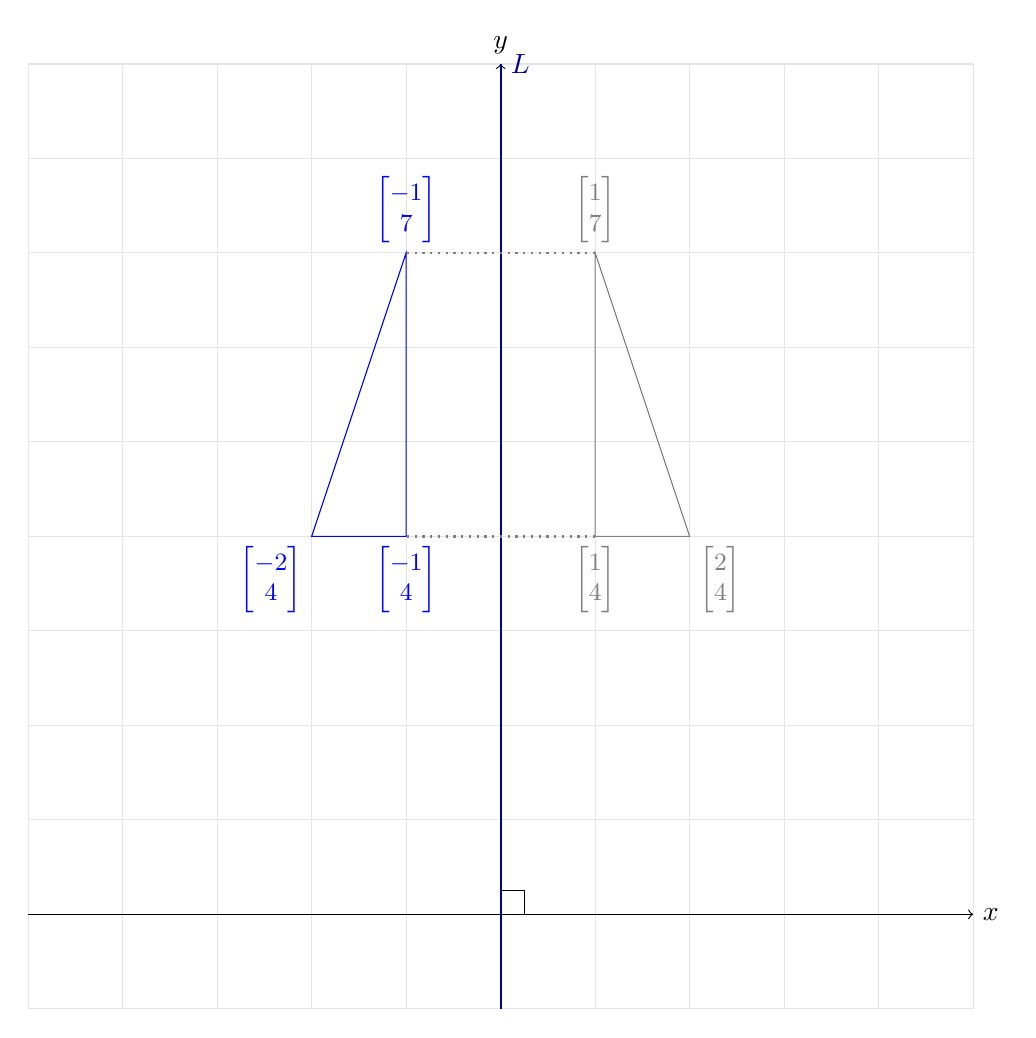
\begin{tikzpicture} [scale = 1.2]
        \coordinate (O) at (0,0);
        \coordinate (xaxis) at (8, 0);
        \coordinate (yaxis) at (0, 8);
        \draw[thin,gray!20] (-5,-1) grid (5,9);
        \draw[->] (-5,0)--(5,0) node[right]{$x$};
        \draw[->] (0,-1)--(0,9) node[above]{$y$};
        \draw [black!40!blue, thick] (0, -1) -- (0, 9) node[anchor=west]{$L$};
        \draw[gray] (1,4) node[anchor=north]{$\small\begin{bmatrix}1\\4\end{bmatrix}$}
            -- (2,4) node[anchor=north west]{$\small\begin{bmatrix}2\\4\end{bmatrix}$}
            -- (1,7) node[anchor=south]{$\small\begin{bmatrix}1\\7\end{bmatrix}$}
            -- cycle;
        \draw[blue] (-1,4) node[anchor=north]{$\small\begin{bmatrix}-1\\4\end{bmatrix}$}
            -- (-2,4) node[anchor=north east]{$\small\begin{bmatrix}-2\\4\end{bmatrix}$}
            -- (-1,7) node[anchor=south]{$\small\begin{bmatrix}-1\\7\end{bmatrix}$}
            -- cycle;
        \draw [gray, thick,dotted] (1,4) -- (-1,4);
        \draw [gray, thick,dotted] (1,7) -- (-1,7);
        \pic [draw, angle radius = .3cm] {right angle = xaxis--O--yaxis};
    \end{tikzpicture}
\end{gather*}

\pagebreak
(g) Draw the triangle formed by the columns of $R_e(\frac{\pi}{4})A$.
\begin{align*}
    R_e\left( \frac{\pi}{4} \right)A &= \begin{bmatrix}
        0&1\\1&0
    \end{bmatrix} \begin{bmatrix}
        1 & 2 & 1\\4 & 4 & 7
    \end{bmatrix}\\&= \begin{bmatrix}
        4 & 4 & 7\\1 & 2 & 1
    \end{bmatrix}
\end{align*}
\begin{gather*}
    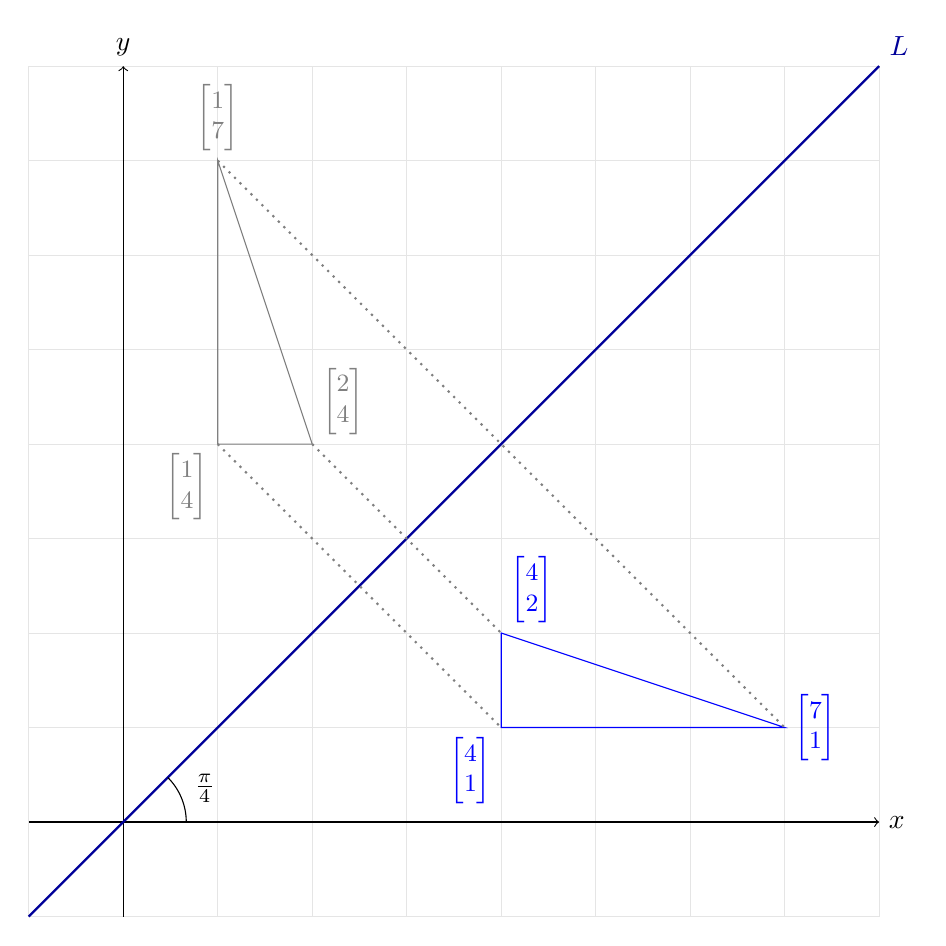
\begin{tikzpicture}[scale = 1.2]
        \coordinate (O) at (0,0);
        \coordinate (xaxis) at (8, 0);
        \coordinate (45) at (8, 8);
        \draw[thin,gray!20] (-1,-1) grid (8,8);
        \draw[->] (-1,0)--(8,0) node[right]{$x$};
        \draw[->] (0,-1)--(0,8) node[above]{$y$};
        \draw[gray] (1,4) node[anchor=north east]{$\small\begin{bmatrix}1\\4\end{bmatrix}$}
            -- (2,4) node[anchor=south west]{$\small\begin{bmatrix}2\\4\end{bmatrix}$}
            -- (1,7) node[anchor=south]{$\small\begin{bmatrix}1\\7\end{bmatrix}$}
            -- cycle;
        \draw[blue] (4,1) node[anchor=north east]{$\small\begin{bmatrix}4\\1\end{bmatrix}$}
            -- (4,2) node[anchor=south west]{$\small\begin{bmatrix}4\\2\end{bmatrix}$}
            -- (7,1) node[anchor=west]{$\small\begin{bmatrix}7\\1\end{bmatrix}$}
            -- cycle;
        \draw [black!40!blue, thick] (-1, -1) -- (8, 8) node[anchor=south west]{$L$};
        \draw [gray, thick,dotted] (1,4) -- (4,1);
        \draw [gray, thick,dotted] (2,4) -- (4,2);
        \draw [gray, thick,dotted] (1,7) -- (7,1);
        \pic [draw, "$\frac{\pi}{4}$", angle eccentricity=1.4, angle radius = .8cm] {angle = xaxis--O--45};
    \end{tikzpicture}
\end{gather*}\\

(h) Describe what $R_e(\theta)$ does.
\paragraph{Solution.}
As you can see, $R_e\left( \theta \right)$ reflects vector $\mathbf{x}$ by a line $L$ whose slope equals to $\tan\theta$ when it is multiplied on the vector $\mathbf{x}$.

\end{document}